\chapter{Introduzione e complementi di algebra lineare}

\section{Che cos'è l'analisi numerica?}

\dfn{Analisi numerica}{
  Sviluppare e analizzare \textit{algoritmi} per risolvere \textit{problemi matematici} (algebra lineare, teoria dei numeri, ottimizzazione, etc.) usando l'\textit{approssimazione numerica}.
}

\nt{In questo corso non si è alla ricerca di soluzioni esatte, ma di soluzioni approssimate.}

\dfn{Calcolo scientifico}{
  Esplorare l'applicazione dei metodi numerici a problemi concreti delle scienze fisiche, dell'ingegneria, delle scienze sociali e della vita, etc.
}
\begin{center}
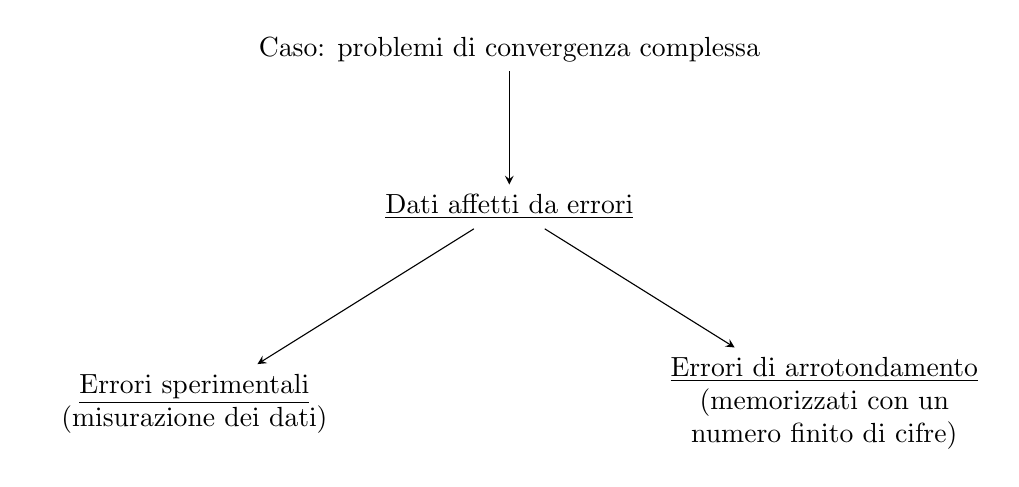
\begin{tikzpicture}[
  level 1/.style={sibling distance=40cm,level distance=2cm},
  level 2/.style={sibling distance=8cm,level distance=2.5cm},
  edge from parent/.style={->,draw},
  >=stealth
  ]
  % Root node
  \node {Caso: problemi di convergenza complessa}
    % First level nodes
  child {node {\underline{Dati affetti da errori}}
      % Second level nodes
      child {node [text width=4cm, align=center]{\underline{Errori sperimentali} \\ (misurazione dei dati)}}
      child {node [text width=4cm, align=center]{\underline{Errori di arrotondamento} \\ (memorizzati con un numero finito di cifre)}}
    };
\end{tikzpicture}
\end{center}
\nt{Gli errori sperimentali sono dovuti alla strumentazione e a errori di misurazione. Gli errori di arrotondamento sono dovuti al fatto che i calcolatori utilizzano un numero finito di cifre quindi i numeri reali $\bbR$ vengono approssimati a numeri razionali $\bbQ$.}

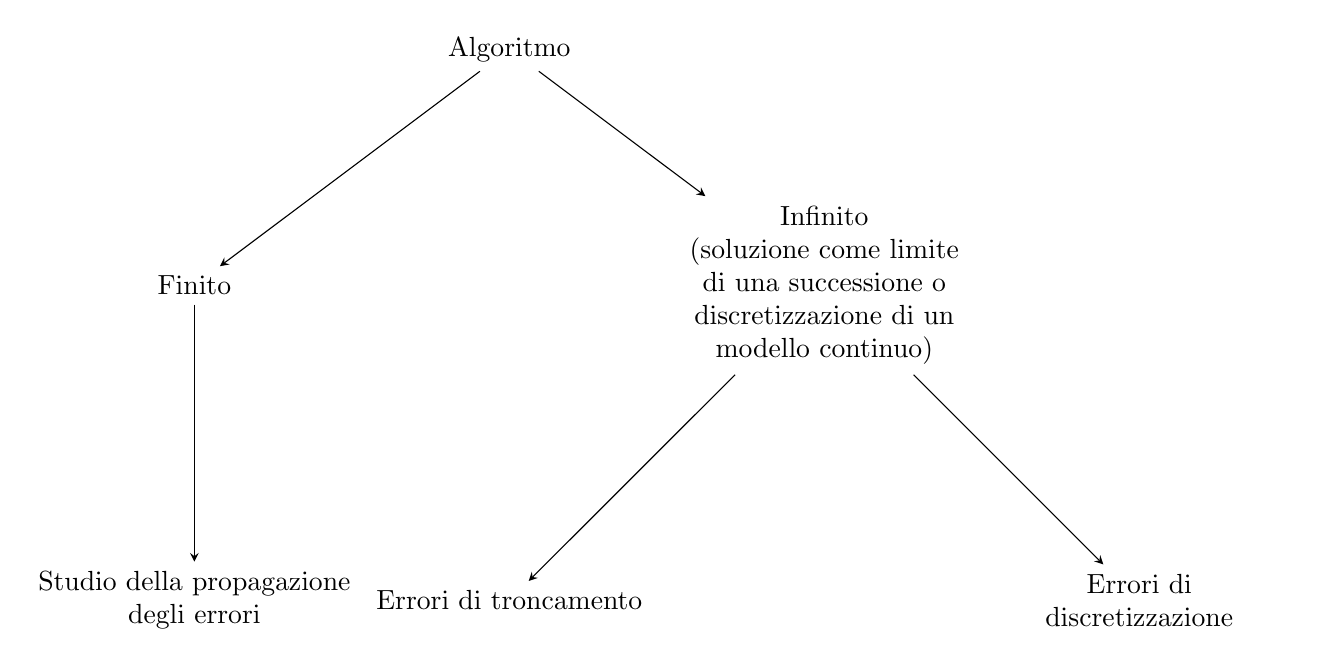
\begin{tikzpicture}[
  level 1/.style={sibling distance=8cm, level distance=3cm},
  level 2/.style={sibling distance=8cm, level distance=4cm},
  edge from parent/.style={->, draw},
  >=stealth
  ]
  % Root node
  \node {Algoritmo}
    % First level nodes
    child {node {Finito}
      child {node  [text width=4cm, align=center]{Studio della propagazione \\ degli errori}}
    }
    child {node  [text width=4cm, align=center]{Infinito \\ (soluzione come limite \\ di una successione o \\ discretizzazione di un \\ modello continuo)}
      child {node {Errori di troncamento}}
      child  [text width=4cm, align=center]{node {Errori di \\ discretizzazione}}
    };

  \end{tikzpicture}

\subsection{Buona posizione e Condizionamento}

Per prevedere l'esito di un fenomeno o simulare l'andamento di un processo si costruisce un \textit{modello matematico}.

\dfn{Modello matematico}{
  Complesso di formule che descrivono il comportamento del fenomeno in esame.
}

\nt{Da un modello/problema matematico si vuole passare a un problema numerico.}

\dfn{Problema numerico}{
  Non tutti i problemi matematici sono effettivamente risolubili. Si introducono semplificazioni o approssimazioni per rendere il problema risolubile numericamente da un calcolatore.
}

\nt{Bisogna notare che si vuole avere a che fare con problemi ben posti\footnote{Visti in "Metodologie e Tecnologie Didattiche per l'Informatica" e "Storia dell'Informatica".}.}

\dfn{Problema ben posto}{
  Ammette \textit{una e una sola} soluzione che dipende dalla \textit{continuità dei dati}. Il caso opposto è un problema mal posto.
}

\ex{Problemi mal posti}{
  \begin{itemize}
    \item [$\Rightarrow$] $x^2 + 1 = 0$, $\not\exists$ soluzione in $\bbR$;
      \item [$\Rightarrow$] $x + y = 1$, $\exists$ infinite soluzioni in $\bbR$.
  \end{itemize}
}

\nt{Un problema e ben posto/mal posto anche in base al tipo di soluzioni che si sta cercando, per esempio il primo esempio ha una soluzione in $\bbC$.}

\dfn{Problema instabile}{
  La soluzione non dipende dalla continuità dei dati. \textit{Piccole perturbazioni} sui dati in ingresso portano a \textit{errori consistenti} sui dati in uscita. Il caso opposto è un problema stabile.
}

\nt{Questo ci porta a parlare di condizionamento di un problema.}

\dfn{Condizionamento del problema}{
  Misura qualitativa di come la soluzione viene influenzata dalla perturbazione dei dati\dots

  Siano $\delta d$ una perturbazione dei dati del problema, $\delta x$ la corrispondente perturbazione sulla sua soluzione e $||\text{°}||$ una qualsiasi \textit{norma vettoriale}.

  \begin{itemize}
    \item $K$ è il numero di condizionamento assoluto, ossia $||\delta x|| \leq K ||\delta d||$;
    \item $K^*$ è il numero di condizionamento relativo, ossia $\frac{||\delta x||}{||x||} \leq K^* \frac{||\delta d||}{||d||}$
  \end{itemize}
}

\nt{Le perturbazioni relative tengono conto della dimensione del dato che si sta perturbando.}

\ex{Perturbazione}{
  Calcolare il numero di condizionamento (relativo) del prodotto tra 2 numeri $x$ e $y$ con perturbazione.

$$|E_x| \leq T$$

$$|E_y| \leq T$$

Prodotto calcolando con dati perturbati (con $E_x E_y$ molto piccolo):

$$x (1 + E_x) y (1 + E_y) = x y (1 + E_x + E_y + E_x E_y) = x y (1 + E_x + E_y) $$

La perturbazione sul prodotto è $E_{xy} = E_x + E_y$ con  $|E_{xy}| = |E_x + E_y| \leq |E_x| + |E_y| \leq 2 T$,
per cui il numero di condizionamento è 2.

}

\subsection{Algoritmi}

\dfn{Algoritmo}{
  Un algoritmo è una \textit{sequenza univoca} di un \textit{numero finito} di \textit{operazioni elementari} che stabilisce come calcolare la soluzione di un problema, assegnati certi dati iniziali.
}

\cor{Sequenza univoca}{
  Formule + Ordine con cui eseguire le operazioni.
}

\cor{Operazioni elementari}{
  Di semplice comprensione.
}

\cor{Numero finito}{
  Se l'algoritmo è iterativo bisogna introdurre almeno un criterio d'arresto. 
}

\cor{Input/Output}{
  Il numero e il tipo di dati richiesti dall'algoritmo e di dati generati da esso.
}

\dfn{Algoritmo stabile}{
  Un algoritmo è stabile quando la successione delle operazioni che lo compone non amplifica eccessivamente gli errori presenti sui dati. Il caso opposto è un algoritmo instabile.  
}

\dfn{Complessità computazionale}{
  In analisi numerica è il numero delle operazioni in virgola mobile (flop) necessarie per risolvere il problema mediante l'algoritmo dato.
}

\nt{In questo corso tratteremo problemi ben posti, ben condizionati e algoritmi stabili con bassa complessità computazionale e occupazione di memoria.}










